%!TEX root = ../wbi.tex
\section{Software Architecture} % (fold)
\label{sec:software_architecture}

\begin{figure*}[t]
  \centering
    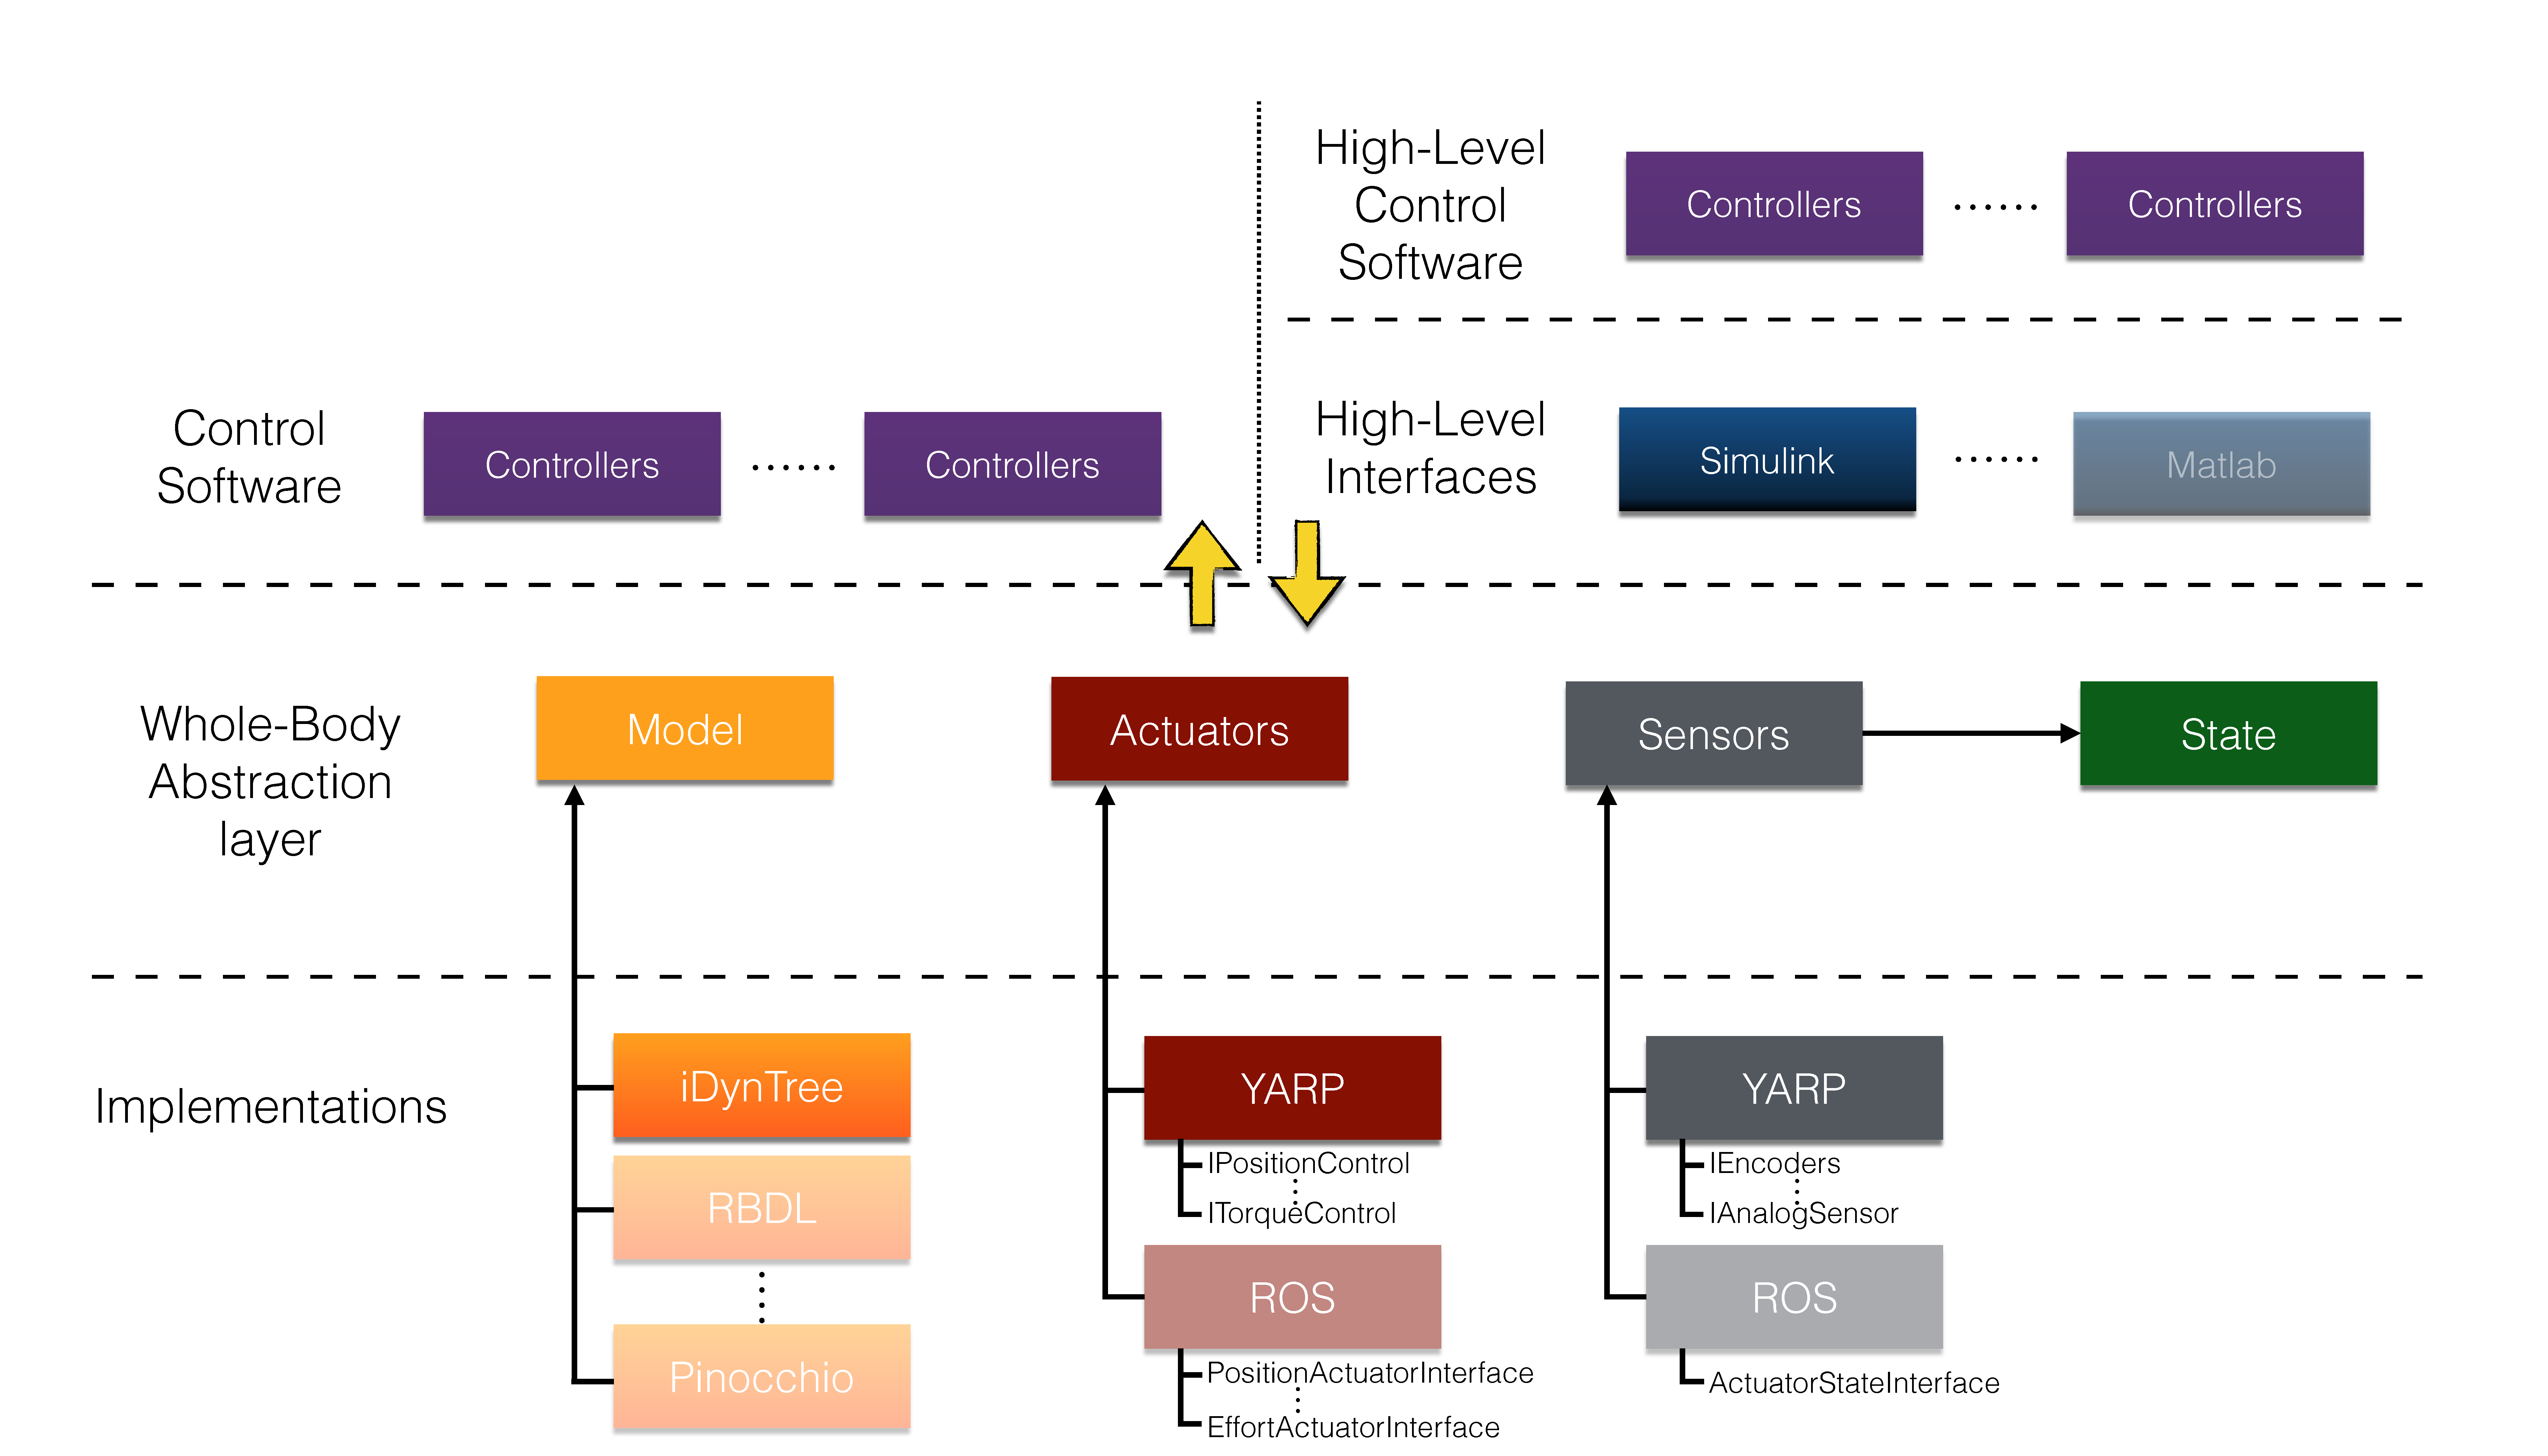
\includegraphics[width=\textwidth]{figs/WBI_diagram}
  \caption{Schema of the proposed whole-body Abstraction layer. Controllers communicate to the kinematic and dynamic library and to the robot software through the proposed library. The implemented elements are drawn with full colour while the shaded blocks represented examples of possible implementations currently unavailable}
  \label{fig:sw_architecture}
\end{figure*}

% \todo[inline]{``Component'' is a quite overloaded concept in Robotics Software Engineering. See
% \cite{brugaliComponent2009,brugaliComponent2010} . Typically it indicates the minimum "block" of computations available in a given robotics framework, for example OROCOS components or ROS Nodes. YARP does not have a real "component", in several aspects both a YARP module or a YARP device could be considered a "Component". Anyhow I don't think we can call this different parts of the libraries "Component".  }

We propose a software abstraction layer to simplify creating whole-body controllers for highly redundant mechanical systems.
Given the requirements introduced in the previous sections we highlight four main elements that must be present in the library, i.e. \emph{Actuators}, \emph{Sensors},  \emph{State} and \emph{Model}.
The abstraction offered by the library allows one to also easily implement higher-level interfaces such as a Simulink\textsuperscript{\textregistered} interface.
Figure~\ref{fig:sw_architecture} summarizes the whole software architecture.

Note that the paradigm described by this library does not assume any particular robot operating system or underlining software as this is left to the actual library implementation.


% \subsection{Library Core} % (fold)
% \label{sub:library_core}
%
% \todo[inline]{I do not understand if the paper until know refers to a generic "decomposition" of the functionality necessary for whole body control (that could be applied to different library/frameworks) or specifically to our WBI stuff. The first hypothesis is nice (if we are able to write it down nicely) but in that case I don't understand why we write that the library should be written in C++. A good example that does that (discussing "general" things and then provide a concrete example) even if in a more complex way is \cite{vanthienen20145c}. }
%
% The core of the library is provided by an abstraction layer implemented in C++.
A crucial feature of the proposed abstraction layer is related to the ordering of the information provided from and to the robot.
In fact, the elements that directly interface the hardware, i.e. the \emph{Actuators}, \emph{Sensors} and \emph{State} have to represent the information in a robot-dependent suitable way.
On the other hand, the \emph{Model} element usually interfaces with libraries that represent the information with the formalism of Eq.~\eqref{eq:system_dynamics}.
To further complicate the problem, the control software may want to access only a subset of the degrees of freedom modelled by the dynamics library, or provided by the robot.
The whole-body abstraction library must thus orchestrate all the various elements to provide a unified interface to the control software.

We now describe in detail the role that each element has in the proposed library.

\subsection{Actuators} % (fold)
\label{sub:actuators}

The \emph{actuators} element abstracts the actual control of the robot motors.
In particular it exposes the possible motors controllable mode, e.g. position control, velocity control and torque control just to cite the most common.
Of course, it also provides the possibility to specify the references for the low level controllers.

% subsubsection actuators (end)

\subsection{Sensors} % (fold)
\label{sub:sensors}

The \emph{sensors} element is the counterpart of the \emph{actuators} element.
In fact, it abstracts all the sensors available on the robot, usually the readings from encoders, force/torque sensors or accelerometers and it is responsible for providing access to the latest sensor measurements.

% subsubsection state (end)

\subsection{State} % (fold)
\label{sub:state}

The \emph{state} element represents all the possible information which can be measured or estimated on the robot.
This implies that \emph{state} encompasses the information provided by the \emph{sensor} element.
Furthermore, it provides additional information which can come from estimation or filtering of the data.
For example, if the robot provides only joint position measurements, e.g. coming from the joint encoders, a first and second derivative filter can provide velocity and acceleration measurements. 
In case this information is provided by the robot itself, no additional processing is required from the interface.
It is important to notice that in both cases the control software using the abstraction library will remain exactly the same.


% subsubsection state (end)

\subsection{Model} % (fold)
\label{sub:model}

The last element is the \emph{model} element.
It abstracts the kinematic- and dynamic-related information that a controller needs while computing the control law.
In general data are represented with the formalism of Eq.~\eqref{eq:system_dynamics}.
Note that a common requirement for a control library is to control only a subset of the degrees of freedom of a robot, e.g. control only the lower body of a legged robot while walking.
For this reason, the library must correctly compute the kinematics and dynamics of the whole system, while considering the possibility to expose only a subset of the quantities as requested by the control software.

% subsubsection model (end)

% section software_architecture (end)
